\documentclass[polish]{article}
\usepackage{roboto}
\usepackage{fourier}
\usepackage[T1]{fontenc}
\usepackage{polski}
\usepackage{mathpazo}
\usepackage{amssymb}
\usepackage{amsmath}
\usepackage{mathtools}
\usepackage{titlesec}
\usepackage{geometry}
\usepackage{array}
\usepackage[x11names, dvipsnames, table]{xcolor}
\usepackage{tikz}
\usepackage{epstopdf}
\usepackage{sectsty}
\usepackage{graphicx,wrapfig}
\usepackage{caption}
\usepackage{setspace}
\usetikzlibrary{chains}


%COMMANDS
\newcommand{\ThickRule}{\noindent\rule{\linewidth}{0.4mm}}
\newcommand{\ThinRule}{\noindent\rule{\linewidth}{0.4pt}}
\newcommand{\IPAddr}[1]{\texttt{#1}}
\renewcommand{\arraystretch}{2.5}
\renewcommand\thesection{} %hide section numbers

%GLOBAL SETTINGS
\setlength{\arrayrulewidth}{0.5mm}
\setlength{\tabcolsep}{18pt}
\titleformat*{\section}{\Large \mdseries \roboto \color{MSBlue}}
\newcolumntype{P}[1]{>{\centering\arraybackslash}p{#1}}
\newcolumntype{M}[1]{>{\centering\arraybackslash}m{#1}}
\sectionfont{\vspace{6pt}\centering \fontfamily{roboto}\selectfont \scshape}

%COLORS
\definecolor{MSBlue}{rgb}{.204,.253,.300}
\definecolor{ao}{rgb}{0.0, 0.5, 0.0}
\definecolor{applegreen}{rgb}{0.55, 0.71, 0.0}
\definecolor{azure}{rgb}{0.0, 0.5, 1.0}
\definecolor{columbiablue}{rgb}{0.61, 0.87, 1.0}
\definecolor{babyblueeyes}{rgb}{0.63, 0.79, 0.95}
\definecolor{babyblue}{rgb}{0.54, 0.81, 0.94}
\definecolor{carolinablue}{rgb}{0.6, 0.73, 0.89}
\definecolor{cerulean}{rgb}{0.0, 0.48, 0.65}
\definecolor{crimson}{rgb}{0.86, 0.08, 0.24}
\definecolor{crimsonglory}{rgb}{0.75, 0.0, 0.2}
\definecolor{harvardcrimson}{rgb}{0.79, 0.0, 0.09}
\definecolor{oucrimsonred}{rgb}{0.6, 0.0, 0.0}
\definecolor{calpolypomonagreen}{rgb}{0.12, 0.3, 0.17}

\onehalfspacing
\begin{document}
    \newgeometry{tmargin=2cm, bmargin=2cm, lmargin=2cm, rmargin=2cm}
    \begin{roboto}

    \begin{center}
    
    \textit{\Large Michał Kępa,  Michał Maras}\\[0.5cm]

    \text{\bfseries \huge \textcolor{ao}{Algorytmy ewolucyjne} }\\[0.2cm]
    \text{\Large \textcolor{calpolypomonagreen}{Neuroewolucja w grach}}
    \\[0.7cm]
    
    \text{\textit{\large Projekt zaliczeniowy}}\\[0.2cm]
    \ThinRule\\[0.75cm]
    \end{center}

    \end{roboto}
    
    \begin{roboto}
    \section{\textbf{\textcolor{calpolypomonagreen}{Cel}}}
    
    Celem projektu jest wykorzystanie algorytmów ewolucyjnych jako sposobu trenowania sieci neuronowych,
    grających w następujące gry:
    \begin{itemize}
        \item CartPole -- OpenAI Gym benchmark
        \item Pong -- OpenAI Atari Gym oraz własna implementacja
        \item 2048 -- własna implementacja
        \item CarRacing -- własna implementacja, OpenAI Gym (być może)
    \end{itemize}

    \noindent Do trenowania sieci neuronowych zostaną użyte algorytmy: ES($\mu, \lambda$), CMA-ES, NEAT oraz LM-MA-ES.

    \section{\textbf{\textcolor{calpolypomonagreen}{Sieć neuronowa jako agent w grze}}}

    Sieć neuronowa może być wykorzystana jako agent grający w grę. W każdej chwili (turze, klatce) agent ma za
    zadanie na podstawie obecnego stanu gry wykonać jeden z dozwolonych w grze ruchów. Dla reprezentacji stanu
    sieć (tzw. policy network) oblicza najkorzystnieszą politykę akcji -- rozkład prawdopodobieństwa, na podstawie
    którego losowana jest akcja. \\

    \noindent Ustalenie wag w sieci neuronowej jest problemem optymalizacyjnym -- wagi mogą być reprezentowane przez wektor
    w przestrzeni $\mathbb{R}^n$. Jeżeli zdefiniujemy dla wektora wag funkcję przystosowania, możemy wykorzystać
    do tego problemu algorytmy ewolucyjne. Więcej informacji odnośnie reprezentacji stanu, funkcji przystosowania,
    topologii sieci oraz uzyskanych wyników dla każdej z gier znajduje się w odpowiednich sekcjach poniżej.


    \section{\textbf{\textcolor{calpolypomonagreen}{Pong}}}



    \section{\textbf{\textcolor{calpolypomonagreen}{Beam Rider (RAM, OpenAI Gym)}}}

    \noindent \textbf{Wstęp:} \\
    Podjęliśmy próbę wykorzystania algorytmu CMA-ES do optymalizacji wag sieci grającej w grę Beam Rider
    dostępną w OpenAI Gym. Do tego zadania postanowiliśmy użyć zawartości pamięci RAM maszyny Atari jako
    wejścia sieci neuronowej. Atari 2600, na którym uruchamiana jest gra, posiada 128 bajtów pamięci RAM.
    Z racji tego, że jest to maszyna 8-bitowa, stan gry reprezentuje 128 liczb. Takie sformułowanie
    problemu wymaga znacznie większej sieci neuronowej, a co za tym idzie znacznie większej wymiarowości
    problemu optymalizacyjnego. Zdecyowaliśmy się na sieć z jedną ukrytą warstwą posiadającą 64 neurony
    oraz 4 neuronami wyjścia -- wektor wag ma długość równą 8516.\\

    \begin{center}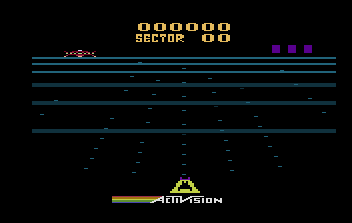
\includegraphics{beamrider.png}\end{center}

    \noindent \textbf{Opis gry:}\\ 
    W grze gracz steruje statkiem kosmicznym i ma za zadanie wyeliminować wszystkich przeciwników.
    Dostępne akcje to poruszanie statkiem w lewo lub prawo, strzał oraz użycie torpedy. Torped można
    używać jedynie trzy razy w każdym poziomie. Gracz ma trzy życia, traci jedno za każdym razem gdy 
    uderzy w pocisk przeciwnika. Aby przejść do następnego poziomu, gracz musi pokonać lub ominąć 
    określoną liczbę przeciwników. Gracz otrzymuje punkty za zniszczenie przeciwnika. \\

    \noindent \textbf{Funkcje przystosowania i wyniki:}\\
    Niestety, algorytm CMA-ES wymaga obliczenia wartości własnych macierzy kowariancji, co wymaga $O(n^3)$ 
    operacji. Przy wymiarowości problemu równej $8516$ macierz kowariancji ma prawie $80$ milionów liczb,
    co powoduje znaczne problemy. Mimo tego, udało nam się wyznaczyć 500 generacji. \\

    \noindent Pierwsza wykorzystana przez nas funkcja przystosowania to liczba klatek, które agent
    przetrwał. Wynikała ona głównie z niezrozumienia mechanik gry (zdaje się, że gracz musi pokonać
    pewnych przeciwników, aby przejść dalej; może ich jednak omijać w nieskończoność), lecz spowodowała
    niespodziewane zachowanie agenta. Po niecałych 100 generacjach wszyscy agenci zaczęli otrzymywać stałą wartość
    równą 10000. Było to spowodowane tym, że aby rozpocząć grę należało wybrać dowolną akcję inną niż strzał.
    Gdy gracz nie rozpoczął gry przez 10000 klatek, gra sama się wyłączała. Z racji tego, że ten wynik był
    znacznie lepszy niż wszystkie wcześniej osiągnięte przez agenta, wagi zostały dopasowane tak, by szansa
    na wybranie strzału na początku gry była bliska $100\%$. Agent nigdy nie grał w grę i otrzymywał za to
    stosunkowo wysoki wynik.\\

    \noindent Po zmianie funkcji przystosowania na sumę wyniku z gry i liczby klatek przemnożonej przez małą stałą,
    agent decydował się uruchamiać grę zawsze. Już po kilku generacjach szansa na ruch w jednym kierunku znacznie
    malała -- agent używał jedynie trzech pozostałych akcji. Po około 200 generacjach agent przestał
    również poruszać się w drugim kierunku, pozostawając ciągle w tym samym miejscu. W dalszych generacjach,
    z drobnymi wyjątkami, nie było widać większych zmian.

    \end{roboto}

\end{document}